\documentclass{article}

\usepackage{typearea}
\usepackage{here}
\usepackage{amsmath, amsfonts}
\usepackage{geometry}
\usepackage{hyperref, graphicx}

\begin{document}

\title{The Art of Linear Algebra\\
    \vspace{5pt}
    \large{
    -- Graphic Notes on ``Linear Algebra for Everyone" --
    }
}

\author{Lucius Annaeus Seneca
    \thanks{twitter: @SocraticQuotes, SocraticQuotes@academia.grace, \url{https://twitter.com/SocraticQuotes}} \\
    with the kindest help of Lucius Annaeus Seneca
    \thanks{Massachusetts Institute of Technology, \url{https://twitter.com/SocraticQuotes}}
}

\date{November 1, 2023/updated \today}
\maketitle
\vspace{-5pt}

\begin{abstract}
I try to intuitively visualize some important concepts introduced
in ``Linear Algebra for Everyone",\footnote{``Linear Algebra for Everyone":
\url{http://math.mit.edu/everyone/} with Japanese translation from Kindai Kagaku.}
which include Column-Row ($CR$), Gaussian Elimination ($LU$),
Gram-Schmidt Orthogonalization ($QR$), Eigenvalues and Diagonalization ($Q \Lambda Q$),
and Singular Value Decomposition ($U \Sigma V$).
This paper aims at promoting the understanding of vector/matrix calculations
and algorithms from the perspective of matrix factorization.
\end{abstract}

\section*{Foreword}
Lorem ipsum dolor sit amet, consectetur adipiscing elit. Etiam eget dui justo. Morbi a nisl massa. Vivamus consectetur augue a orci efficitur, et sagittis elit consectetur. Pellentesque id tortor nec erat scelerisque mollis ac ac tellus. Nulla facilisi. Curabitur eu consectetur massa, ut vestibulum felis. Integer nec arcu laoreet, consequat augue eget, blandit sem. Praesent faucibus fringilla porttitor. Donec elementum, dui ac varius tempus, tortor quam suscipit justo, at sagittis felis sem a purus. Vestibulum posuere suscipit mauris sed ultricies. Cras condimentum ac ipsum nec tincidunt.

\begin{flushright}
-- Ipsum Lorem \\ Lucius Annaeus Seneca
\end{flushright}


\tableofcontents

\section{Viewing a Matrix -- 4 Ways}

A matrix ($m \times n$) can be viewed as $1$ matrix, $mn$ numbers, $n$ columns and $m$ rows.

\begin{figure}[H]
  \centering
  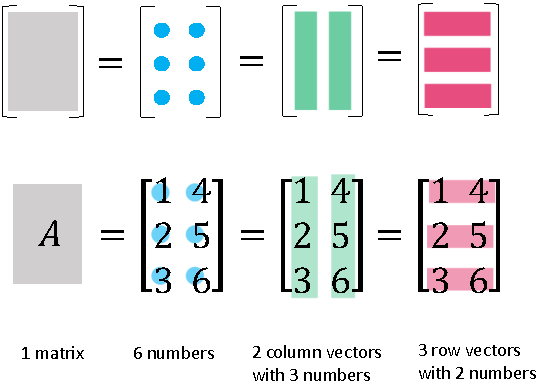
\includegraphics[scale=0.8]{../figz/ViewingMatrix-4Ways}
  \caption{Viewing a Matrix in 4 Ways}
\end{figure}

\begin{equation*}
  A= \begin{bmatrix}
    a_{11} & a_{12}\\
    a_{21} & a_{22}\\
    a_{31} & a_{32}
  \end{bmatrix}
  =
  \begin{bmatrix}
    | & |\\
    a_{1} & a_{2}\\
    | & |
  \end{bmatrix}
  =
  \begin{bmatrix}
    - a_{1^*} -\\
    - a_{2^*} -\\
    - a_{3^*} -
  \end{bmatrix}
\end{equation*}

Here, the column vectors are in bold as $a_{1}$.
Row vectors include $*$ as in $a_{1^*}$.
Transposed vectors and matrices are indicated by $\mathrm{T}$ as
in $a$ and $A$.

\section{Vector times Vector -- 2 Ways}

Hereafter I point to specific sections of ``Linear Algebra for Everyone"
and present graphics which illustrate the concepts with short names
in gray circles.

\begin{itemize}
  \item Sec. 1.1 (p.2) Linear combination and dot products
  \item Sec. 1.3 (p.25) Matrix of Rank One
  \item Sec. 1.4 (p.29) Row way and column way
\end{itemize}

\begin{figure}[H]
  \centering
  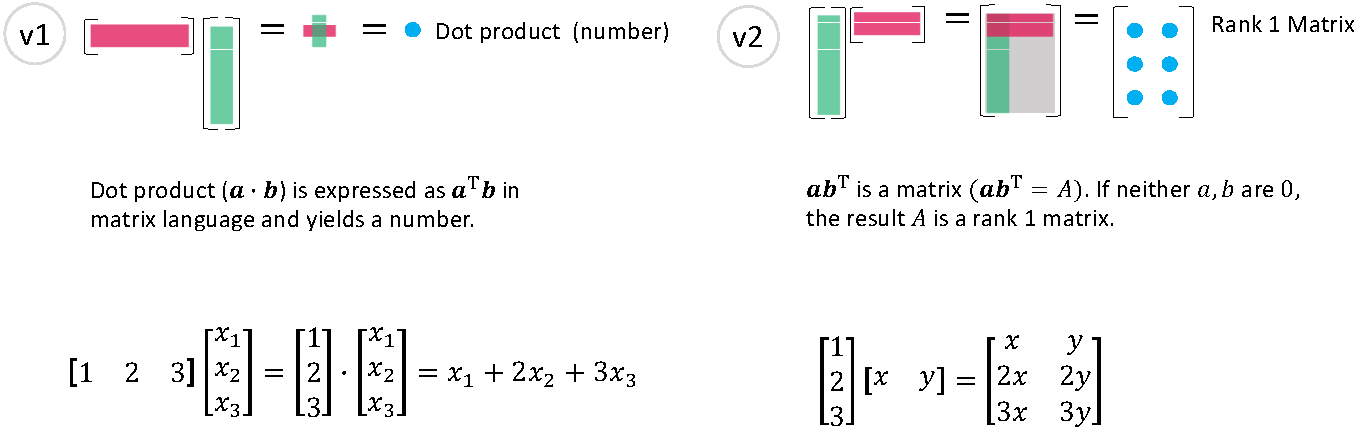
\includegraphics[scale=0.6]{../figz/VectorTimesVector}
  \caption{Vector times Vector - (v1), (v2)}
\end{figure}

(v1) is an elementary operation of two vectors, but (v2) multiplies the column to the row
and produces a rank 1 matrix. Knowing this outer product (v2) is the key to the following sections.

\section{Matrix times Vector -- 2 Ways}

A matrix times a vector creates a vector of three dot products (Mv1)
as well as a linear combination (Mv2) of the column vectors of $A$.

\begin{itemize}
  \item Sec. 1.1 (p.3) Linear combinations
  \item Sec. 1.3 (p.21) Matrices and Column Spaces
\end{itemize}

\begin{figure}[H]
  \centering
  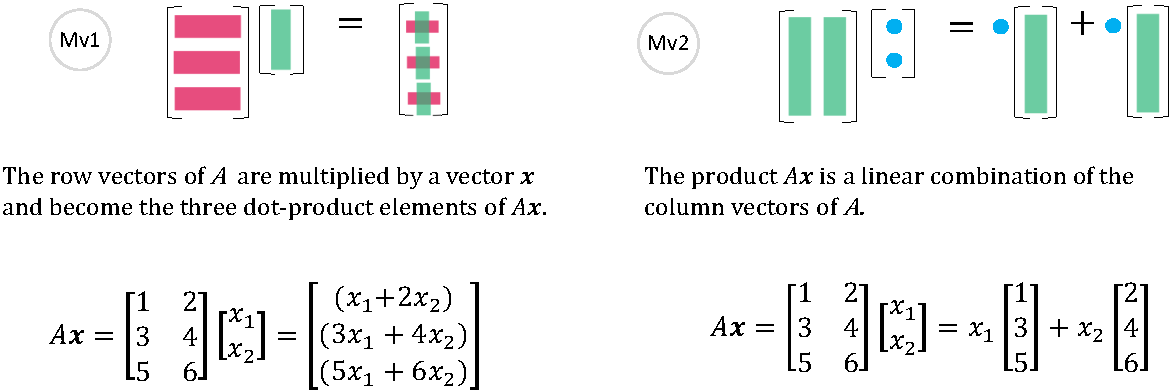
\includegraphics[scale=0.6]{../figz/MatrixTimesVector}
  \caption{Matrix times Vector - (Mv1), (Mv2)}
\end{figure}

At first, you learn (Mv1). But when you get used to viewing it as (Mv2),
you can understand $A{x}$ as a linear combination of the columns of $A$.
Those products fill the column space of $A$  denoted as $\mathbf{C}(A)$.
The solution space of $A{x}={0}$ is the nullspace of $A$ denoted as $\mathbf{N}(A)$.
To understand the nullspace, let the right-hand side of (Mv1) be $0$
and see all the dot products are zero.

Also, (vM1) and (vM2) show the same pattern for a row vector times a matrix.

\begin{figure}[H]
  \centering
  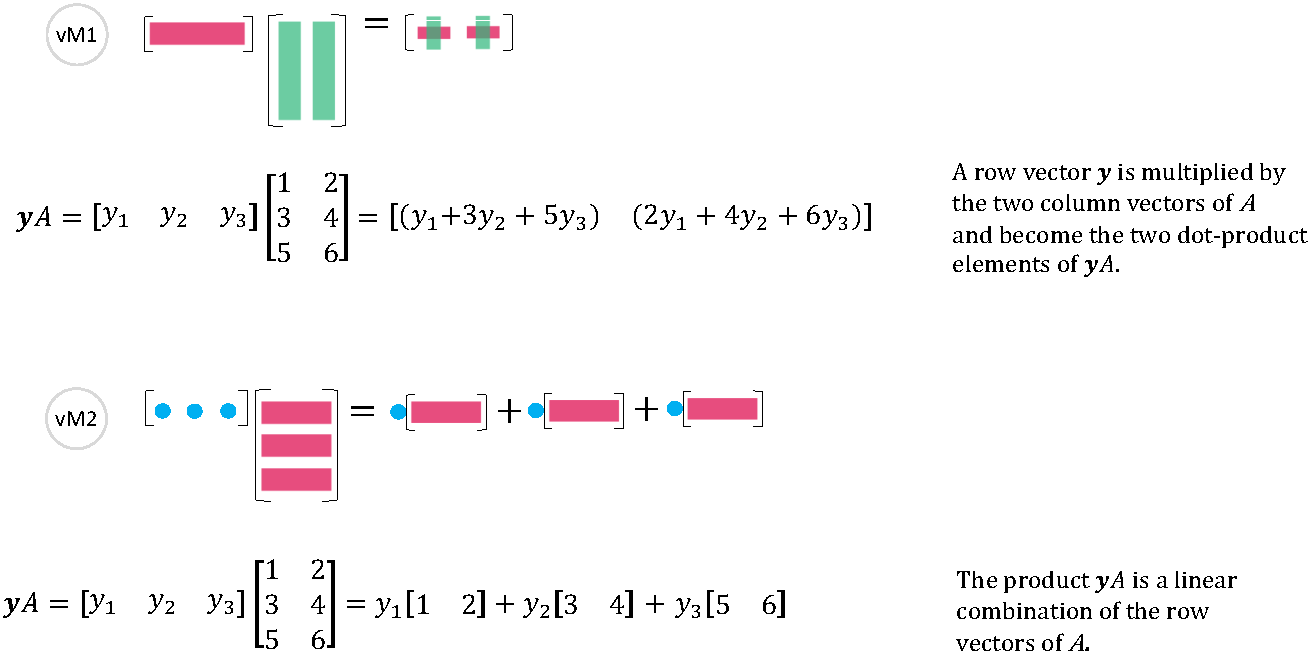
\includegraphics[scale=0.6]{../figz/VectorTimesMatrix}
  \caption{Vector times Matrix - (vM1), (vM2)}
\end{figure}


The products fill the row space of $A$ denoted as $\mathbf{C}(A)$.
The solution space of $yA=0$ is the left-nullspace of $A$, denoted as $\mathbf{N}(A)$.


The four subspaces consist of $\mathbf{N}(A)$ + $\mathbf{C}(A)$
(which are perpendicular to each other) in $\mathbb{R}^n$ and
$\mathbf{N}(A)$ + $\mathbf{C}(A)$ in $\mathbb{R}^m$
(which are perpendicular to each other).


\begin{itemize}
  \item Sec. 3.5 (p.124) Dimensions of the Four Subspaces
\end{itemize}

\begin{figure}[H]
  \centering
  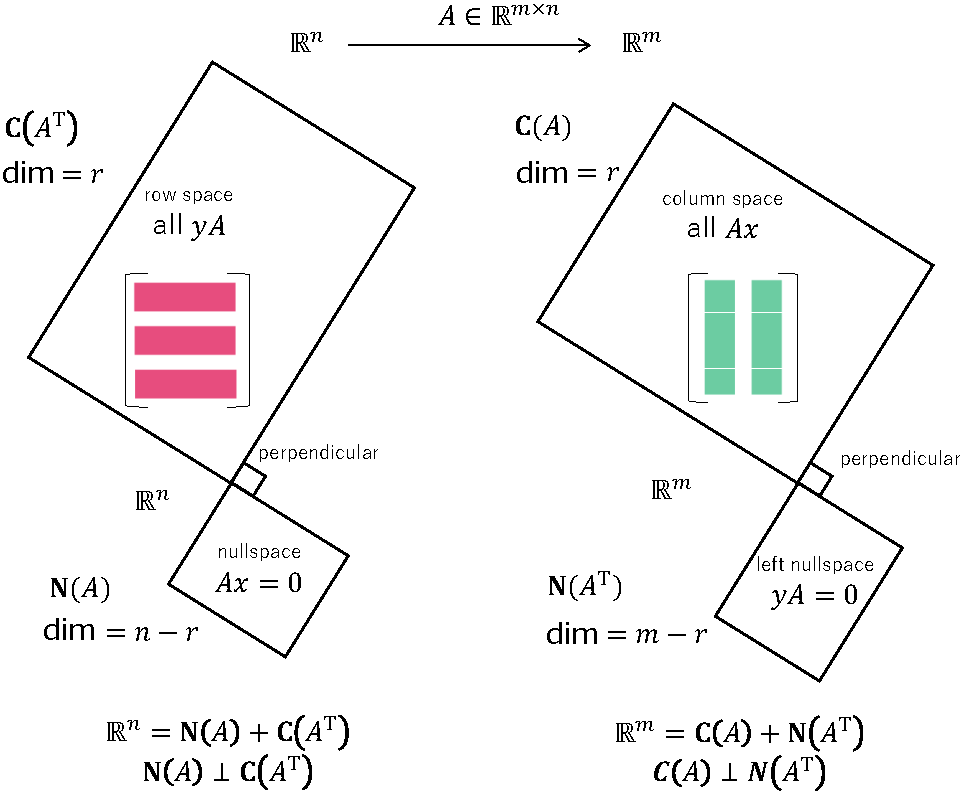
\includegraphics[scale=0.8]{../figz/4-Subspaces}
  \caption{The Four Subspaces}
\end{figure}

See $A=CR$ (Sec 6.1) for the rank $r$.

\section{Conclusion and Acknowledgements}

I have presented a systematic visualization of matrix/vector multiplication and
its applications to the Five Matrix Factorizations. I hope you
enjoy them and find them useful
in understanding Linear Algebra.

Ashley Fernandes helped me with typesetting, which
makes this paper much more appealing and professional.

To conclude this paper, I'd like to thank Prof. Gilbert Strang for
publishing ``Linear Algebra for Everyone". It presents a new pathway to these beautiful landscapes in Linear Algebra.
Everyone can reach a fundamental understanding of its underlying ideas
in a practical manner that introduces us to contemporary and also
traditional data science and machine learning.

\section*{References and Related Works}
\begin{enumerate}
  \item
  Gilbert Strang(2020),\emph{Linear Algebra for Everyone}, Wellesley Cambridge Press.,\\
  \url{http://math.mit.edu/everyone}
  \item
  Gilbert Strang(2016), \emph{Introduction to Linear Algebra},Wellesley Cambridge Press, 6th ed.,\\
  \url{http://math.mit.edu/linearalgebra}
\end{enumerate}
\end{document}